\section{\acrfull{scgs}}
\label{sec:scgs}

So far we have presented the set of differential equations that govern the fluid flow, and we have also discretized them using the FVM and applying different schemes (for the convection and diffusion terms).

In the following we will discuss the \acrfull{scgs} method by \cite[Vanka (1986)]{VANKA1986138}, which combine all the information we have presented so far, and will allow us to solve the discretized equations iteratively.

Notice that when we say \textit{solve the equations}, we mean to find the values of the velocity components and the pressure at each cell of the domain, namely $U(x_i, y_j)$ \& $V(x_i, y_j)$ \& $P(x_i, y_j)$, so to have a complete description of the flow field.

\subsection{Variable Correction Concept}
\label{subsec:variable_correction_concept}

Before presenting the \acrshort{scgs} method itself, it's now useful to introduce the concept of variable correction, which is crucial for the understanding of the method.

The idea here is to observe a generic current state of the system $\phi^{(n)}$, as the sum of a known part $\phi^{(n-1)}$ and a correction $\delta \phi^{(n)}$:

\begin{equation}
    \phi^{(n)} = \phi^{(n-1)} + \delta \phi^{(n)}
    \label{eq:variable_correction_concept}
\end{equation}

Where $\phi$ is a generic variable, and $n$ is the iteration index.

For simplicity of notation, we will drop the iteration index in the following, and we will rewrite Equation \ref{eq:variable_correction_concept} as:

\begin{equation}
    \phi = \phi^* + \phi'
    \label{eq:variable_correction_concept_simplified}
\end{equation}

Where $\phi^*$ is the known part, and $\phi'$ is the correction.

By doing so, we can rewrite the state of the system at the current iteration as:

\begin{align}
    u_{i,j} & = u_{i,j}^* + u_{i,j}' \\
    v_{i,j} & = v_{i,j}^* + v_{i,j}' \\
    p_{i,j} & = p_{i,j}^* + p_{i,j}'
    \label{eq:variable_corrections}
\end{align}
\subsection{Equations Coupling}
\label{subsec:equations_coupling}

At this point, one could ask how the three equations we have presented so far are related to each other.
The answer is in the continuity equation, which is the key to couple the velocity and pressure fields (and indeed, have a close form of the system with 3 equations \ref{eq:INS_steady_2D_discretized_continuity_final} \ref{eq:INS_steady_2D_discretized_momentum_x_final} \ref{eq:INS_steady_2D_discretized_momentum_y_final} and 3 unknowns).

Given that the continuity equation is defined for a given $p-CV$ and that involve the all the four velocity components at the faces of the control volume, it should be intuitive that in order to solve the equilibrium across one cell, we need to have a system of equations that involve all the four velocity components.

By recalling the representation with index notation for the $p-CV$, we can compose our system of equations.

\begin{figure}[H]
    \centering
    \def\nCV{1}
    \def\dX{5cm}
    \def\dY{5cm}

    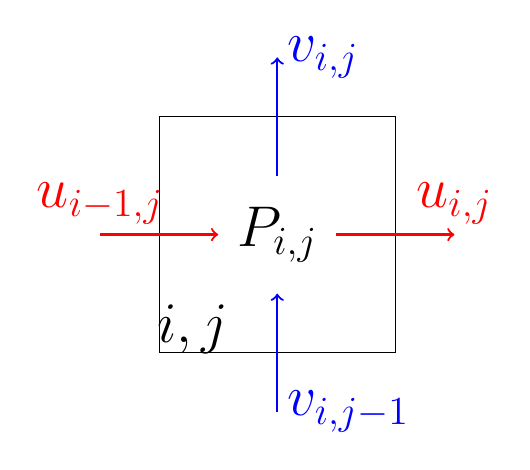
\begin{tikzpicture}[every node/.style={font=\huge}]

        \draw (0, 0) -- ++(\dX, 0) -- ++(0, \dY) -- ++(-\dX, 0) -- cycle;

        \node at (\dX/2, \dY/2) {$P_{i,j}$};
        \draw[thick, red, ->] (\dX/2, \dY/2)++(\dX/4, 0) -- ++(\dX/2, 0) node[pos=1, above] {$u_{i,j}$};
        \draw[thick, red, ->] (\dX/2, \dY/2)++(-\dX/2-\dX/4, 0) -- ++(\dX/2, 0) node[pos=0, above] {$u_{i-1,j}$};
        \draw[thick, blue, ->] (\dX/2, \dY/2)++(0,  \dY/4) -- ++(0, \dY/2) node[pos=1, right] {$v_{i,j}$};
        \draw[thick, blue, ->] (\dX/2, \dY/2)++(0, -\dY/2-\dY/4) -- ++(0, \dY/2) node[pos=0, right] {$v_{i,j-1}$};

        \node at (\dX/7, \dY/10) {$i,j$};

    \end{tikzpicture}
    \caption{Generic $p-CV$ with the velocity components at the faces.}
\end{figure}

\begin{equation}
    \begin{cases}
        \text{Mom. } u_{i-1, j} \\
        \text{Mom. } u_{i, j}   \\
        \text{Mom. } v_{i, j-1} \\
        \text{Mom. } v_{i, j}   \\
        \text{Con.}
    \end{cases}
    =
    \begin{cases}
        (A_P^u)_{i-1,j} u_{i-1,j}                                       & = \sum_{nb} (A_{nb}^u)_{i-1,j} (u_{nb})_{i-1,j} + (p_{i-1,j} - p_{i,j}) \Delta y \\
        (A_P^u)_{i,j} u_{i,j}                                           & = \sum_{nb} (A_{nb}^u)_{i,j} (u_{nb})_{i,j} + (p_{i,j} - p_{i+1,j}) \Delta y     \\
        (A_P^v)_{i,j-1} v_{i,j-1}                                       & = \sum_{nb} (A_{nb}^v)_{i,j-1} (v_{nb})_{i,j-1} + (p_{i,j-1} - p_{i,j}) \Delta x \\
        (A_P^v)_{i,j} v_{i,j}                                           & = \sum_{nb} (A_{nb}^v)_{i,j} (v_{nb})_{i,j} + (p_{i,j} - p_{i,j+1}) \Delta x     \\
        (u_{i,j} - u_{i-1,j}) \Delta y + (v_{i,j} - v_{i,j-1}) \Delta x & = 0
    \end{cases}
\end{equation}

The system of equations is composed by 5 equations and 5 unknowns ($u_{i-1,j}$, $u_{i,j}$, $v_{i,j-1}$, $v_{i,j}$, $p_{i,j}$), and it's the result of the coupling of the momentum and continuity equations across a generic $p-CV$.
\subsection{Residual Concept}
\label{subsec:residual_concept}

Being the \acrshort{scgs} an iterative method, it's crucial to introduce the concept of residual, which is the key to understand the convergence of the method.

The residual is the difference between the left-hand side and the right-hand side of the discretized equations, and it's a measure of the error of the current state of the system.

For our system of 5 equations, we can define 5 residuals, one for each equation.

To simplify the set of equations (and have a simpler matrix resolution afterwards), we can choose to apply the correction to only some variables, and not to all of them.

In particular, we can choose to neglect the correction for the velocity and pressure components regarding the neighbor cells, and apply the correction only to the pressure and the velocity components at the current cell.

By doing so, we can rewrite the system of equations as:

\begin{gather}
    (A_P^u)_{i-1,j} (u_{i-1,j}^*+u_{i-1,j}') = \sum_{nb} (A_{nb}^u)_{i-1,j} (u_{nb}^*)_{i-1,j} + (p_{i-1,j}^* - (p_{i,j}^* + p_{i,j}')) \Delta y \\
    (A_P^u)_{i,j}   (u_{i,j}  ^*+u_{i,j}')   = \sum_{nb} (A_{nb}^u)_{i,j} (u_{nb}^*)_{i,j}     + ((p_{i,j}^* + p_{i,j}') - p_{i+1,j}^*) \Delta y   \\
    (A_P^v)_{i,j-1} (v_{i,j-1}^*+v_{i,j-1}') = \sum_{nb} (A_{nb}^v)_{i,j-1} (v_{nb}^*)_{i,j-1} + (p_{i,j-1}^* - (p_{i,j}^* + p_{i,j}')) \Delta x \\
    (A_P^v)_{i,j}   (v_{i,j}  ^*+v_{i,j}')   = \sum_{nb} (A_{nb}^v)_{i,j} (v_{nb}^*)_{i,j}     + ((p_{i,j}^* + p_{i,j}') - p_{i,j+1}^*) \Delta x   \\
    ((u_{i,j}  ^*+u_{i,j}') - (u_{i-1,j}^*+u_{i-1,j}')) \Delta y + ((v_{i,j}  ^*+v_{i,j}') - (v_{i,j-1}^*+v_{i,j-1}')) \Delta x = 0
\end{gather}

As explained in Subsection \ref{subsec:variable_correction_concept}, the $^*$ superscript is used to indicate the value of the variable at the previous iteration, and the $'$ superscript is used to indicate the correction to apply to the variable.
This means that the $\phi^*$ are known values, and the $\phi'$ are the unknowns to solve for.

We can now rearrange each equation to have the unknowns on the left-hand side and the known on the right-hand side:

\begin{align}
    (A_P^u)_{i-1,j} u_{i-1,j}' + p_{i,j}' \Delta y                      & = R^u_{i-1,j} \\
    (A_P^u)_{i,j}   u_{i,j}'   - p_{i,j}'   \Delta y                    & = R^u_{i,j}   \\
    (A_P^v)_{i,j-1} v_{i,j-1}' + p_{i,j}' \Delta x                      & = R^v_{i,j-1} \\
    (A_P^v)_{i,j}   v_{i,j}'   - p_{i,j}'   \Delta x                    & = R^v_{i,j}   \\
    (u_{i,j}' - u_{i-1,j}') \Delta y + (v_{i,j}' - v_{i,j-1}') \Delta x & = R^c_{i,j}
    \label{eq:residual_system}
\end{align}

Where $R^\phi_{i,j}$ is the residual of the $\phi$ equation at the $i,j$ cell.

The residuals, computed from the previous system by moving the known terms to the right-hand side, are defined as:

\begin{align}
    R^u_{i-1,j} & = \sum_{nb} (A_{nb}^u)_{i-1,j} (u_{nb}^*)_{i-1,j} - (A_P^u)_{i-1,j} u_{i-1,j}^*   + (p_{i-1,j}^* - p_{i,j}^*) \Delta y \\
    R^u_{i,j}   & = \sum_{nb} (A_{nb}^u)_{i,j} (u_{nb}^*)_{i,j} - (A_P^u)_{i,j} u_{i,j}^*           + (p_{i,j}^* - p_{i+1,j}^*) \Delta y \\
    R^v_{i,j-1} & = \sum_{nb} (A_{nb}^v)_{i,j-1} (v_{nb}^*)_{i,j-1} - (A_P^v)_{i,j-1} v_{i,j-1}^*   + (p_{i,j-1}^* - p_{i,j}^*) \Delta x \\
    R^v_{i,j}   & = \sum_{nb} (A_{nb}^v)_{i,j} (v_{nb}^*)_{i,j} - (A_P^v)_{i,j} v_{i,j}^*           + (p_{i,j}^* - p_{i,j+1}^*) \Delta x \\
    R^c_{i,j}   & = -\left[(u_{i,j}^* - u_{i-1,j}^*) \Delta y + (v_{i,j}^* - v_{i,j-1}^*) \Delta x\right]
\end{align}


\subsection{Gauss-Seidel Iterative Method}
\label{subsec:gauss_seidel_iterative_method}

Before, proceeding with the solution of the \acrshort{scgs} method, we need to introduce the \acrfull{gs} method.

The \acrshort{gs} method is an iterative method used to solve a system of linear equations, and it's based on the idea of solving one equation at a time, and using the updated values of the variables to solve the next equation.

For our purpose, is interesting to observe how the introduction of the 'under-relaxation' factor $\alpha$ can help to improve the convergence of the method.

In particular, we can apply the \acrshort{gs} method to solve a similar equation of our system, as for example:

\begin{equation}
    (A_P^\phi) \phi_P = \sum_{nb} (A_{nb}^\phi) \phi_{nb} + S^\phi
\end{equation}

Where $\phi$ is a generic variable, and $S^\phi$ is the source term of the equation.

The \acrshort{gs} method can be written as:

\begin{align}
    \phi_P & = \frac{\sum_{nb} (A_{nb}^\phi) \phi_{nb}^* + S^\phi}{A_P^\phi} + \phi_P^*                                \\
    \phi_P & = \alpha \left(\frac{\sum_{nb} (A_{nb}^\phi) \phi_{nb}^* + S^\phi}{A_P^\phi} - \phi_P^*\right) + \phi_P^*
\end{align}

Where $\phi_P^*$ is the value of the variable at the previous iteration, and $\alpha$ is the under-relaxation factor.

By rearranging the last equation, we have:

\begin{equation}
    \phi_P' = \frac{R_P^\phi}{\left(\frac{A_P^\phi}{\alpha_\phi}\right)}
\end{equation}

Where $\phi_P'$ is the correction to apply to the variable, and $R_P^\phi$ is the residual of the equation at the $P$ cell.

This result will be useful in the next section.

\subsection{Vanka's approach}
\label{subsec:vanka_approach}

The \acrshort{scgs} method is based on the idea of solving the equations in a coupled way.

This means that for each iteration, we will obtain the correction for each of the 5 variables simultaneously.
To make this possible, we need to introduce a new matrix, called the \textbf{Vanka matrix \cite{VANKA1986138}}.

Considering the system of equations \ref{eq:residual_system}, we can write them in a matrix form as:

\begin{equation}
    \begin{bmatrix}
        (A_P^u)_{i-1,j} & 0             & 0               & 0             & \Delta y  \\
        0               & (A_P^u)_{i,j} & 0               & 0             & -\Delta y \\
        0               & 0             & (A_P^v)_{i,j-1} & 0             & \Delta x  \\
        0               & 0             & 0               & (A_P^v)_{i,j} & -\Delta x \\
        -\Delta y       & \Delta y      & -\Delta x       & \Delta x      & 0
    \end{bmatrix}
    \begin{bmatrix}
        u'_{i-1,j} \\
        u'_{i,j}   \\
        v'_{i,j-1} \\
        v'_{i,j}   \\
        p'_{i,j}
    \end{bmatrix}
    =
    \begin{bmatrix}
        R_{i-1,j}^u \\
        R_{i,j}^u   \\
        R_{i,j-1}^v \\
        R_{i,j}^v   \\
        R_{i,j}^c
    \end{bmatrix}
    \label{eq:vanka_matrix}
\end{equation}

As we can see, the Vanka matrix is a $5 \times 5$ matrix, and it's a function of the coefficients of the discretized equations, and of the grid spacing.

Our unknown is the vector of the corrections, being the $A_P^\phi$ coefficients and the $R^\phi$ residuals known from the previous iteration.

Given that, we can solve the system of equations \ref{eq:vanka_matrix} to obtain the corrections for the velocity and pressure components at each cell of the domain.

To do so, we must invert the Vanka matrix, and multiply it by the residuals vector:

\begin{equation}
    \begin{bmatrix}
        \phi'
    \end{bmatrix}
    =
    \begin{bmatrix}
        A^\phi
    \end{bmatrix}^{-1}
    \begin{bmatrix}
        R^\phi
    \end{bmatrix}
\end{equation}

As stated in \cite{VANKA1986138}, the inverse of the Vanka matrix can be computed analytically using the following algorithm:

\begin{gather}
    r_i = \frac{a_{5i}}{a_{ii}}, \quad i = 1, 2, 3, 4 \\
    DEN = \sum_{i=1}^{4} a_{5i} r_i \\
    x_5 = \frac{\left[\sum_{i=1}^{4} r_i b_i - b_5\right]}{DEN} \\
    x_i = \frac{b_i - a_{i5} x_5}{a_{ii}}, \quad i = 1, 2, 3, 4
\end{gather}

Where $a_{ij}$ are the elements of the Vanka matrix $A^\phi$, $b_i$ are the elements of the residuals vector $R^\phi$, and $x_i$ are the elements of the corrections vector $\phi'$.

In case we want to apply an under-relaxation factor to the corrections, we can modify Vanka's Matrix as follows:

\begin{equation}
    \begin{bmatrix}
        \frac{(A_P^u)_{i-1,j}}{\alpha_u} & 0                              & 0                                & 0                              & \Delta y  \\
        0                                & \frac{(A_P^u)_{i,j}}{\alpha_u} & 0                                & 0                              & -\Delta y \\
        0                                & 0                              & \frac{(A_P^v)_{i,j-1}}{\alpha_v} & 0                              & \Delta x  \\
        0                                & 0                              & 0                                & \frac{(A_P^v)_{i,j}}{\alpha_v} & -\Delta x \\
        -\Delta y                        & \Delta y                       & -\Delta x                        & \Delta x                       & 0
    \end{bmatrix}
\end{equation}

Where $\alpha_u$ and $\alpha_v$ are the under-relaxation factors for the velocity components $u$ and $v$ respectively.
\subsection{Boundary conditions for Lid-Driven Cavity problem}
\label{subsec:boundary_conditions_for_lid_driven}

So far, we have presented all the tools and concepts required to solve a generic fluid flow problem (except for the algorithm itself) that respect the hypothesis and conditions stated at the beginning of Section \ref{sec:derivation_of_discretized_governing_equations}.

In this section we will present the boundary conditions that will be used to solve the Lid-Driven Cavity problem and their implementation inside the \acrshort{scgs} method.



\subsubsection{Ghosts cells}

Consider that our domain has already been discretized (subdivided) into $N_x \times N_y$ cells.

If we think of the scheme for both the convection and diffusion presented before, we can see that at the boundary of our domain, the coefficients $A_p\phi$ \ref{tab:Ap_coefficients} involve cells that are outside the domain.
For this reason, we need to add a layer of cells outside the physical domain, called ghost cells, to calculate the coefficients at the boundary.

The number of ghost cells required depends on the order of the scheme used to calculate the coefficients. For a second-order scheme, we need at least one ghost cell, and for a fourth-order scheme, we need at least two ghost cells.

Here, and also in the implementation of the \acrshort{scgs} method in the code, we will consider the possibility to adopt a mixed strategy scheme and use:

\begin{itemize}
    \item Away from boundaries: higher-order schemes
    \item Near boundaries: \acrshort{uds} scheme for convection and 2nd-order scheme for diffusion
\end{itemize}

By doing so, we ensure that at the boundaries both the schemes will be applicable with just a single layer of ghost cells.

\begin{figure}[H]
    \centering
    \def\nCV{5}
    \def\dX{1.5cm}
    \def\dY{1.5cm}

    \begin{tikzpicture}

        \foreach \n in {0,1,...,\nCV}
            {
                \draw (0, \n*\dY) -- (\nCV*\dX, \n*\dY);
                \draw (\n*\dX, 0) -- (\n*\dX, \nCV*\dY);
            }

        % \foreach \n in {0,1,...,\the\numexpr\nCV-1\relax}
        %     {
        %         \draw[dashed] (-\dX/2, \n*\dY + \dY/2) -- (\nCV*\dX+\dX/2, \n*\dY + \dY/2);
        %         \draw[dashed] (\n*\dX + \dX/2, -\dY/2) -- (\n*\dX + \dX/2, \nCV*\dY+\dY/2);
        %     }

        \foreach \y in {0,1,...,\the\numexpr\nCV-1\relax}
            {
                \foreach \x in {0,1,...,\the\numexpr\nCV-1\relax}
                    {
                        \node[font=\small] at (\x*\dX+\dX/6, \y*\dY+\dY/10) {$_{\the\numexpr\x+0\relax,\the\numexpr\y+0\relax}$};
                    }
            }

        \draw[line width=0.5mm] (\dX, \dY) -- (\dX, \nCV*\dY-\dY) -- (\nCV*\dX-\dX, \nCV*\dY-\dY) -- (\nCV*\dX-\dX, \dY) -- cycle;

        % \fill[red, opacity=0.1] (0, 0) rectangle (\nCV*\dX, \nCV*\dY);
        \fill[yellow, opacity=0.3] (\dX, \dY) rectangle (\nCV*\dX-\dX, \nCV*\dY-\dY);

    \end{tikzpicture}
    \caption{Physical domain and ghost cells}
    \label{fig:ghost_cells}
\end{figure}

In Figure \ref{fig:ghost_cells}, the yellow area represents the physical domain, while the frame surrounding it represents the ghost cells.

As we can see, the indexes of the cells stick to the physical domain, while the ghost cells may have negative indexes.

In the case above, we can declare some of the problem that will be recalled during the following sections:

\begin{itemize}
    \item Physical domain: $N_x \times N_y$ grid. In the example above, $N_x = N_y = 3$
    \item Physical domain indexes: from $(1,1)$ to $(3,3)$. In general, from $(1,1)$ to $(N_x,N_y)$.
    \item Ghost cells layer: may have different sizes along the $x$ and $y$ directions. In the example above, the ghost cells layer has a size of $N_g = 1$ cell in both directions. We will stick with this size for the rest of the document.
    \item Ghost cells indexes: may have negative indexes. In the example above, the ghost cells have indexes from $(0,0)$ to $(4,4)$, that is equivalent to $(1-N_g,1-N_g)$ to $(N_x+2*N_g-1,N_y+2*N_g-1)$.
\end{itemize}

We can now proceed to identify the boundary conditions for the Lid-Driven Cavity problem.



\subsubsection{No-slip condition}

As boundary conditions for the Lid-Driven Cavity problem (and for most of the fluid flow problems), we have the no-slip condition, which gives us the constraint for two direction of the velocity field:

\begin{itemize}
    \item Component normal to the wall: given a condition of impenetrability, the velocity component normal to the wall must be zero (no-penetration)
    \item Component tangential to the wall: given a condition of no-slip, the velocity component tangential to the wall must equal to the wall velocity
\end{itemize}

As an example, we can consider the cell in position $(1, N_y)$, which is the top-left corner of the physical domain (Figure \ref{fig:ghost_cells} for reference).

\begin{figure}[H]
    \centering
    \def\nCV{2}
    \def\dX{3cm}
    \def\dY{3cm}

    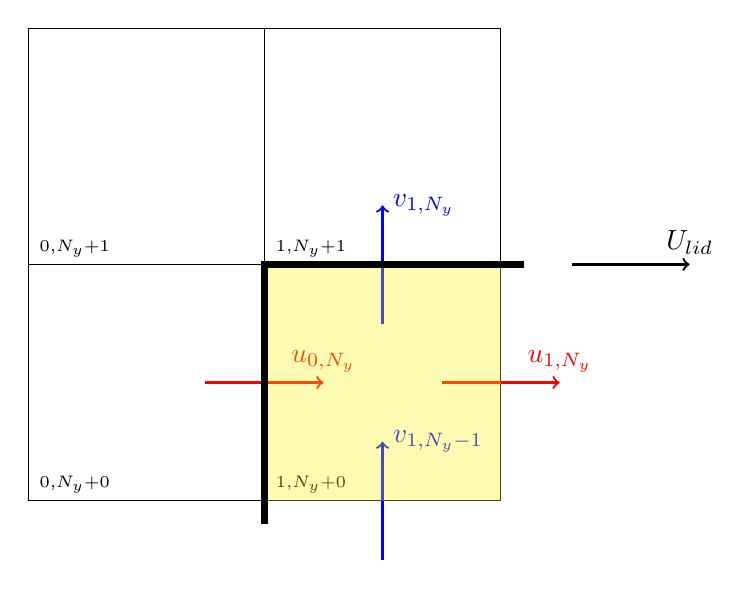
\begin{tikzpicture}

        \foreach \n in {0,1,...,\nCV}
            {
                \draw (0, \n*\dY) -- (\nCV*\dX, \n*\dY);
                \draw (\n*\dX, 0) -- (\n*\dX, \nCV*\dY);
            }

        \foreach \y in {0,1,...,\the\numexpr\nCV-1\relax}
            {
                \foreach \x in {0,1,...,\the\numexpr\nCV-1\relax}
                    {
                        \node[font=\small] at (\x*\dX+\dX/5, \y*\dY+\dY/15) {$_{\x, N_y+\y}$};
                    }
            }

        \draw[thick, blue, ->] (3/2*\dX, 1/2*\dY)++(0,  \dY/4) -- ++(0, \dY/2) node[pos=1, right] {$v_{1,N_y}$};
        \draw[thick, blue, ->] (3/2*\dX, 1/2*\dY)++(0, -\dY/2-\dY/4) -- ++(0, \dY/2) node[pos=1, right] {$v_{1,N_y-1}$};
        \draw[thick, red, ->] (3/2*\dX, 1/2*\dY)++(\dX/4, 0) -- ++(\dX/2, 0) node[pos=1, above] {$u_{1,N_y}$};
        \draw[thick, red, ->] (3/2*\dX, 1/2*\dY)++(-\dX/2-\dX/4, 0) -- ++(\dX/2, 0) node[pos=1, above] {$u_{0,N_y}$};

        \fill[yellow, opacity=0.3] (\dX, 0) rectangle (2*\dX, \dY);

        \draw[line width=1mm] (\dX, -\dY/10) -- (\dX, \dY) -- (2*\dX+\dX/10, \dY);
        \draw[thick, ->] (2*\dX +\dX/10, \dY) ++(\dX/5, 0) -- ++(\dX/2, 0) node[pos=1, above] {$U_{lid}$};

    \end{tikzpicture}
    \caption{Boundary conditions for the cell $(1, N_y)$}
    \label{fig:boundary_conditions_1Ny}
\end{figure}

In this case, we must accomplish the following conditions:

\begin{itemize}
    \item $u_{0, N_y} = 0$ (no-penetration)
    \item $v_{1, N_y} = 0$ (no-penetration)
    \item $u_{1, N_y} = U_{lid}$ (no-slip)
\end{itemize}

Intuitively, we can understand that similar conditions must be applied to the other walls of the domain given the correction of the indexes and the direction of the velocity field.

In general, we can state that the boundary conditions for the Lid-Driven Cavity problem are:

\begin{itemize}
    \item Bottom wall: $v_{i,0} = 0$ (no-penetration) + $u_{i,1} = 0$ (no-slip)
    \item Left wall: $u_{0,j} = 0$ (no-penetration) + $v_{1,j} = 0$ (no-slip)
    \item Top wall: $v_{i,N_y} = 0$ (no-penetration) + $u_{i,N_y} = U_{lid}$ (no-slip)
    \item Right wall: $u_{N_x,j} = 0$ (no-penetration) + $v_{N_x,j} = 0$ (no-slip)
\end{itemize}

We can now proceed to see how these conditions are accounted for in the \acrshort{scgs} method.



\subsubsection{Boundary conditions inside \acrshort{scgs} method}

By adopting the \acrshort{scgs} method, we can impose the boundary conditions in the following way:

\begin{itemize}
    \item No-penetration condition: impose specific coefficients in the Vanka matrix to be zero
    \item No-slip condition: impose specific velocity values in the ghost cells
\end{itemize}

Moreover, as we are going to see, the no-penetration condition imply the velocity to be null and can be imposed to the system before solving the linear system of equations.
Instead, given the mathematical formulation of the no-slip condition, we can impose the velocity values in the ghost cells only after solving the linear system of equations (and will affect the next iteration).

\paragraph{No-penetration condition}

The no-penetration condition imply the normal velocity component at the boundary to be null.
This means that if we start from an initial guess of the velocity field equal to zero everywhere, we must ensure that correction of the velocity field at the boundary is null for each iteration.

Taken for example the cell $(1, N_y)$ as in Figure \ref{fig:boundary_conditions_1Ny}, we know that we must impose $u_{0, N_y} = 0$ \& $v_{1, N_y} = 0$, which means that the correction of the velocity field at the boundary must be null as well $u_{0, N_y}' = 0$ \& $v_{1, N_y}' = 0$.

By recalling the formulation for both the continuity and momentum equations, we can see that multiple terms must be canceled out (known null solution).

For the \textbf{continuity equation} written at the cell $(1, N_y)$, we have:

\begin{equation}
    -u_{0, N_y}' \Delta y + u_{1, N_y}' \Delta y - v_{1, N_y-1}' \Delta x + v_{1, N_y}' \Delta x = R_{1, N_y}^c
\end{equation}

By imposing $[A^\phi]_{5,1} = \Delta y = 0$, we can cancel out the first term, and by imposing $[A^\phi]_{5, 4} = \Delta x = 0$, we can cancel out the third term.

In this way, even if we are not imposing the no-penetration condition directly, we are imposing an equivalent condition that will lead to the same result.

More in general, given the physical domain of size $N_x \times N_y$, we can impose the no-penetration condition for the continuity equation by setting:

\begin{align}
    @i=1, u_{i-1, j}' = 0 \rightarrow [A^\phi]_{5,1} & = - \Delta y = 0 \quad \forall j = 1,2,...,N_y \\
    @i=N_x, u_{i, j}' = 0 \rightarrow [A^\phi]_{5,2} & = \Delta y = 0 \quad \forall j = 1,2,...,N_y   \\
    @j=1, v_{i, j-1}' = 0 \rightarrow [A^\phi]_{5,3} & = - \Delta x = 0 \quad \forall i = 1,2,...,N_x \\
    @j=N_y, v_{i, j}' = 0 \rightarrow [A^\phi]_{5,4} & = \Delta x = 0 \quad \forall i = 1,2,...,N_x
\end{align}

For the \textbf{momentum equations}, written at the cell $(1, N_y)$ for the two components that are controlled by the no-penetration condition, we have:

\begin{align}
    (A_P^u)_{0,N_y} u_{0,N_y}' + p_{0,N_y}' \Delta y & = R^u_{0,N_y} \\
    (A_P^v)_{1,N_y} v_{1,N_y}' - p_{1,N_y}' \Delta x & = R^v_{1,N_y}
\end{align}

By imposing $[A^\phi]_{1,5} = \Delta y = 0$ and $[R^\phi]_{1} = 0$, we can cancel out the first equation, and by imposing $[A^\phi]_{4,5} = - \Delta x = 0$ and $[R^\phi]_{4} = 0$, we can cancel out the second equation.

More in general, given the physical domain of size $N_x \times N_y$, we can impose the no-penetration condition for the momentum equations by setting:

\begin{align}
    @i=1, u_{i-1, j}' = 0 \rightarrow [A^\phi]_{1,5} & = \Delta y = 0 \quad \forall j = 1,2,...,N_y   \\
    @i=N_x, u_{i, j}' = 0 \rightarrow [A^\phi]_{2,5} & = - \Delta y = 0 \quad \forall j = 1,2,...,N_y \\
    @j=1, v_{i, j-1}' = 0 \rightarrow [A^\phi]_{3,5} & = \Delta x = 0 \quad \forall i = 1,2,...,N_x   \\
    @j=N_y, v_{i, j}' = 0 \rightarrow [A^\phi]_{4,5} & = - \Delta x = 0 \quad \forall i = 1,2,...,N_x
\end{align}

\paragraph{No-slip condition}

The idea behind the no-slip condition for the tangential velocity component is to impose the velocity field in the ghost cells so that the interpolation with the velocity field in the physical domain gives the correct value at the boundary.

As an example, we can consider the cell $(1, N_y)$ as in Figure \ref{fig:boundary_conditions_1Ny}.

We know that we must impose $u_{1, N_y} = U_{lid}$.
Given that the condition can't be imposed directly to the correction term as for the no-penetration condition, here we have to solve the system and then impose the condition over the ghost cells velocity based on the current solution of the velocity field.

In particular, we can think of the wall velocity as the average of the velocity in the ghost cell and the velocity in the physical domain.
This implies to impose the following condition for the cell $(1, N_y)$:

\begin{equation}
    U_{lid} = \frac{1}{2} (u_{1, N_y} + u_{1, N_y+1}) \rightarrow u_{1, N_y+1} = 2 U_{lid} - u_{1, N_y}
\end{equation}

More in general, given the physical domain of size $N_x \times N_y$, we can impose the no-slip condition for the velocity field by setting:

\begin{align}
    @i=1, v_{0, j}       & = - v_{1, j} \quad \forall j = 1,2,...,N_y             \\
    @i=N_x, v_{N_x+1, j} & = - v_{N_x, j} \quad \forall j = 1,2,...,N_y           \\
    @j=1, u_{i, 0}       & = - u_{i, 1} \quad \forall i = 1,2,...,N_x             \\
    @j=N_y, u_{i, N_y+1} & = 2 U_{lid} - u_{i, N_y} \quad \forall i = 1,2,...,N_x
\end{align}
\subsection{Convergence criterion}
\label{sec:convergence_criterion}

Being the \acrshort{scgs} method an iterative method, we need to define a criterion to stop the iterations, and to consider the solution as converged.

We could have adopted many criteria, but probably the most intuitive one is to monitor the residuals of the equations over the entire domain for each iteration, and to stop the cycle when the maximum of the residual is below a certain threshold.

So far we have defined 5 residuals, one for each equation, and we can define other 3 residuals derived from the previous ones, as follows:

\begin{equation}
    \begin{aligned}
        \text{Continuity residual} & : R^p = | R^c |                                               \\
        \text{Momentum residual u} & : R^u = \frac{\left( | R_{i-1}^u | + | R_{i}^u | \right) }{2} \\
        \text{Momentum residual v} & : R^v = \frac{\left( | R_{j-1}^v | + | R_{j}^v | \right) }{2}
    \end{aligned}
\end{equation}

By doing so, our convergence criterion will be:

\begin{equation}
    \max \left( R^p, R^u, R^v \right) < \varepsilon
\end{equation}

Where $\varepsilon$ is the threshold and may vary between $10^{-3}$ and $10^{-6}$, depending on the problem and the computational resources available.

